\section{Integrating \xxx into virtual machine} \label{sec:vm-integration}

Primary-backup (\eg, \remus~\cite{remus:nsdi08}), a dominant Virtual Machine 
(VM) fault-tolerance approach, works in a physical time slot manner. In each 
slot, it runs a service in the primary VM to process client requests, tracks 
updated VM states (\eg, dirty memory pages), and buffers network outputs. 
At the end of a slot, a synchronization operation is invoked to transfer dirty 
pages from the primary to backup. Once the transfer succeeds, network outputs 
are sent to clients. By doing so, primary-backup approach ensures 
\emph{external consistency}~\cite{remus:nsdi08}: primary and backup have the 
same states and a primary failure will not be observed by clients.

Unfortunately, despite much effort~\cite{remus:nsdi08,qemu-mc, 
sartakov2017multi,lu2012speculative, gerofi2011rdma}, achieving fast and 
multi-core scalable VM fault-tolerance remains an open 
problem~\cite{dong2013colo,gerofi2011rdma,sartakov2017multi}. There are two main 
reasons for this. One is that the primary-backup approach often has to transfer 
an excessive amount of dirty memory pages, which greatly degrades the 
performance of a service and occupies prohibitive network bandwidth. The other 
reason is that primary-backup approach suffers from the notorious 
``split-brain'' problem~\cite{scales2010design}, in which both the primary and 
backup think itself as the primary when network partition happens and 
therefore break external consistency to the clients.

To address the problems mentioned above, we propose Virtualized \smr (\vsmr), a 
new \smr approach that can achieve fast, multi-core scalable VM fault-tolerance. 
\vsmr enforces same total order of network inputs for a VM replicated across 
hosts. It then periodically invokes a synchronization operation to efficiently 
compute updated page hashes, to compare them across the replicas, and to 
transfer only the divergent pages. Because all the replicas run the same 
code and receive the same network inputs, their memory states should be 
largely the same in a synchronization operation and accordingly the amount of 
data to be transferred for memory state synchronization is expected to be small.

In a conceptual level, \vsmr replicates an entire guest VM as a state machine 
and achieves the strengths of both \smr and primary-backup. By transferring 
only those divergent pages, \vsmr automatically and efficiently ensures 
external consistency. Leveraging the powerful fault-tolerance of \paxos, \vsmr
tackles the ``split-brain problem" in primary-backup systems.

We implemented \yyy, a prototype of \vsmr system in Linux. \yyy leverages 
\xxx \paxos system. \yyy intercepts inbound network packets in the KVM QEMU 
hypervisor~\cite{qemu} and replicates them to other VM hypervisors using \paxos. 
\yyy's synchronization operation is built on top of \paxos for robustness, and 
it uses RDMA to efficiently compare page hashes across replicas.

\yyy develops several optimizations for improving the performance, including  
efficient determination of slot boundary and concurrent 
computation of dirty page hashes.

Similar to primary-backup for ensuring external consistency, \yyy leader must 
buffer all outbound packets before a synchronization operation succeeds, 
including client responses and TCP ACKs. Client programs will stop sending new 
packets when their TCP congestion windows are met, even server programs have 
finished processing requests and become idle. This leads to unnecessary time 
slots. To avoid this, \yyy develops an adaptive-slot algorithm by inserting 
synchronization operations when its leader determines idle status of programs 
running in guest VM.

We also leveraged multi-core hardware and implemented a multi-threaded dirty 
page hash computing mechanism. The mechanism detects the number of CPU cores on 
local host creates same number of threads to compute hashes of dirty physical 
pages since the last synchronization operation.

We evaluated \yyy on 11 widely used programs, including 8 server programs 
(\redis~\cite{redis}, \ssdb~\cite{ssdb}, \mediatomb~\cite{mediatomb}, 
\nginx~\cite{nginx}, \mysql~\cite{mysql}, \tomcat~\cite{tomcat}, 
\pgsql~\cite{pgsql}, and \mongoose~\cite{mongoose}) and 3 dynamic 
language interpreters (\php, \python, and \jsp). To be close to real-world 
deployments, we group these programs into 7 practical services, 
including \cms~\cite{django:cms}, a large, sophisticated content management 
system (CMS) consisting of \nginx, \python, and \mysql.

\begin{figure}[htbp]
\centering
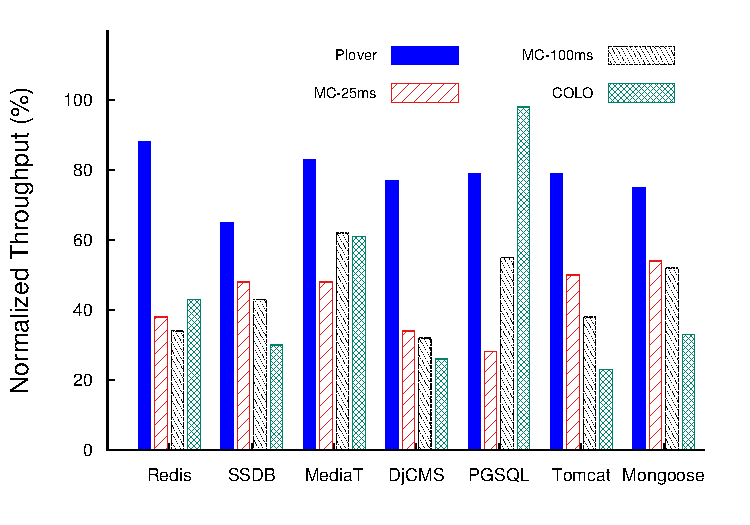
\includegraphics[width=3in]{figures/FIG1__throughput-overhead}
\caption{{\em Throughputs normalized to unreplicated executions (4 vCPUs per 
VM)}. 100\% means no overhead.}
\label{fig:vmtput}
\end{figure}

\begin{figure}[htbp]
\centering
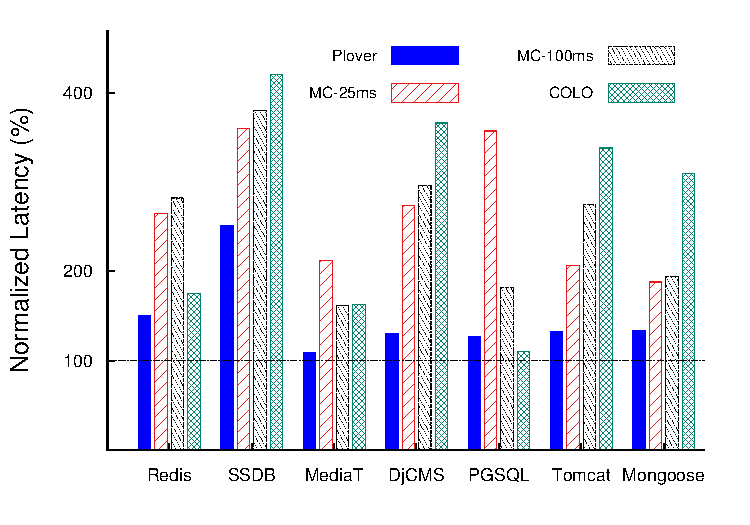
\includegraphics[width=3in]{figures/FIG9_latency-overhead}
\caption{{\em Response times normalized to unreplicated 
executions (4 vCPUs per VM)}. 100\% means no overhead.}
\label{fig:latency}
\end{figure}

For \redis and \ssdb, each request contains a batch of 1K operations 
of 50\% SET and 50\% GET; for the other five services, each request contains 
one operation. We found sending operations in batches for \redis and \ssdb made 
them reach peak throughput. For instance, when each request for \redis contains 
only one SET or GET operation, \redis's throughput is only 43K operation/s for 
32 connections; when each request is a 1K-operation batch, its throughput 
reaches a peak value of 451K operation/s for 32 connections.

We compared \yyy with two fault-tolerance systems:
QEMU-MicroCheckpoint~\cite{qemu-mc} (for short, \qemumc),  a \remus-based 
primary-backup system carried in QEMU~\cite{qemu}; and 
\colo~\cite{dong2013colo}, a primary-backup system acquired and deployed by 
Huawei~\cite{fusionsphere}. \qemumc has an RDMA 
implementation~\cite{qemu-mc-rdma}, but it is being actively developed and 
not runnable on our hosts. We did not use \remus because 
it was built before 2008 and did not run on our hosts. \colo runs the same 
service on both primary and backup, compares per-connection network outputs, 
and does a synchronization if any connection's output diverges.

Figure~\ref{fig:vmtput} shows \yyy, \qemumc, and \colo's throughput on 
7 services. All results are normalized to unreplicated executions ran 
in \kvm because the actual throughputs of different services largely vary. 
\qemumc includes results for both the 25\ms-slot (\remus's default) and 
100\ms-slot (\qemumc's default).
All experiments ran on 4-vCPU per VM (unless specified) because 
\colo~\cite{dong2013colo} and \remus~\cite{remus:nsdi08} evaluated up to 4 
vCPUs per VM. On average, \yyy's throughput is \avgtput higher than \qemumc and 
\colo.

\pgsql is the only service that \yyy is slower than \colo. \colo compares 
per-connection outputs between its primary and backup, and it 
skips transferring memory if outputs did not diverge. \pgsql ran SQL 
transaction workloads and its outputs were mostly the same. Except for 
\pgsql, \yyy was several times faster than \colo. 

To analyze \colo, we also looked into \ssdb, which 
had concurrent SET/GET requests. We found that \colo's output divergence 
was frequent when data dependencies exist among connections (\ie, GET 
requests frequently got different responses when SET and GET requests on the 
same key arrived at \ssdb concurrently). When any output in any connection 
had an output divergence, \colo did a synchronization operation. \colo 
evaluation shows that it greatly slowed down when the number of client 
connections was large. \yyy is not sensitive to outputs.

Figure~\ref{fig:latency} shows the response time of the four systems normalized 
to unreplicated executions. For five services (excluding \redis and \ssdb), 
\xxx's overhead of response time follows the same trend as the 
overhead of throughput because each client connection in these five services 
sends requests one by one. For \redis and \ssdb, because the requests arrive in 
batches in order to saturate the two services, all four systems incur 
high overhead on response time. Specifically, \yyy incurred the highest latency
overhead for \ssdb, because it had a low same dirty page rate of 
77\%. 

Figure~\ref{fig:bandwidth} explains why \yyy's performance was higher. 
\yyy consumes \avgbandwidth less bandwidth than both \qemumc
and \colo on average. This reduction makes \yyy the first VM fault-tolerance 
system that supports consolidating multiple VMs on a host.

\begin{figure}[htbp]
\centering
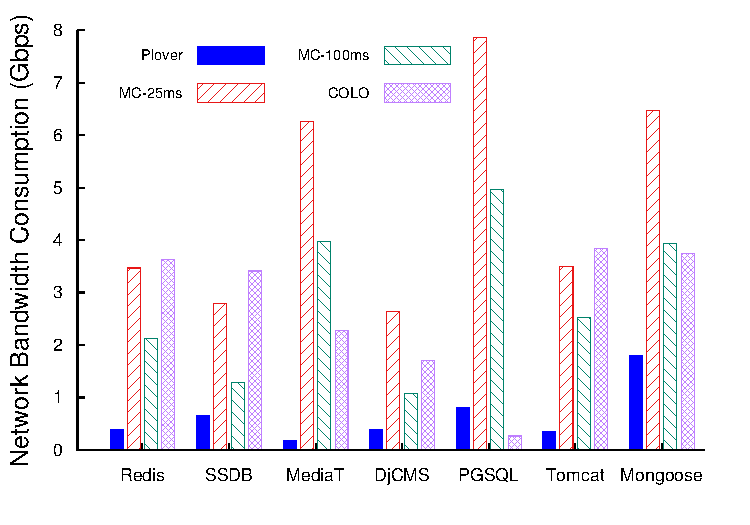
\includegraphics[width=3in]{figures/FIG2__network_bandwidth}
\caption{{\em \yyy network bandwidth consumption compared with \qemumc and 
\colo (all used four vCPUs per VM)}.}
\label{fig:bandwidth}
\end{figure}
